
%(BEGIN_QUESTION)
% Copyright 2011, Tony R. Kuphaldt, released under the Creative Commons Attribution License (v 1.0)
% This means you may do almost anything with this work of mine, so long as you give me proper credit

In this process, raw maple syrup is heated by steam to evaporate water and make it more concentrated.  The control of sugar concentration is much better when the feed flow rate is stable, and so a ``surge tank'' has been added to the front of the process to allow the raw syrup feed rate to vary over time without forcing the evaporator feed rate to fluctuate.  In fact, the surge tank even allows operators to add raw syrup in discrete batches while the system maintains a steady flow rate to the evaporator:

$$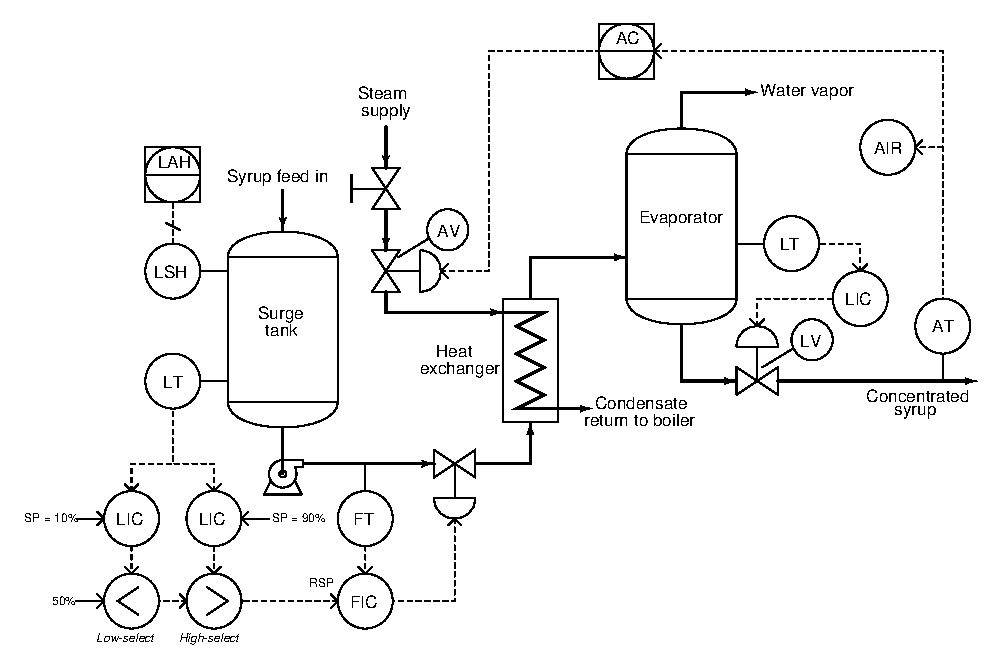
\includegraphics[width=15.5cm]{i00425x01.eps}$$

Examine this control strategy, and then explain how it works, using a series of ``thought experiments'' to demonstrate its action for multiple process conditions.

\vskip 20pt \vbox{\hrule \hbox{\strut \vrule{} {\bf Suggestions for Socratic discussion} \vrule} \hrule}

\begin{itemize}
\item{} For those who have studied PID tuning, explain why the two level controllers on the surge tank {\it must} have absolutely no integral action in them, but rather need to be proportional-only with moderate gain values and fixed bias values of 50\%.
\item{} Predict the effects from one of the transmitters in this system failing with either a high or a low signal.
\end{itemize}

\underbar{file i00425}
%(END_QUESTION)





%(BEGIN_ANSWER)


%(END_ANSWER)





%(BEGIN_NOTES)

Assuming that the two override level controllers have gains of 2 and 50\% bias values makes the thought experiment easier to follow.  Consider the case where surge tank level is 50\%:

$$\includegraphics[width=15.5cm]{i00425x02.eps}$$

\vskip 10pt

Now consider when the surge tank level is 95\%:

$$\includegraphics[width=15.5cm]{i00425x03.eps}$$

\vskip 10pt

Now consider when the surge tank level is 5\%:

$$\includegraphics[width=15.5cm]{i00425x04.eps}$$


\vfil \eject

\noindent
{\bf Prep Quiz:}

Explain the purpose of this {\it surge tank} level/flow control system:

$$\includegraphics[width=15.5cm]{i00425x05.eps}$$

\begin{itemize}
\item{} Control the surge tank level at a constant setpoint value by varying the flow rate
\vskip 5pt 
\item{} Prevent over-heating of the syrup inside the surge tank by tightly regulating flow
\vskip 5pt 
\item{} Maintain a steady flow rate unless the surge tank level goes too high or too low
\vskip 5pt 
\item{} Maintain flow rate at 10\% or at 90\% depending on the level inside the surge tank
\vskip 5pt 
\item{} Regulate flow rate at a constant setpoint regardless of the surge tank level
\vskip 5pt 
\item{} Maintain surge tank at 10\% or at 90\% depending on the flow control setpoint
\end{itemize}


%INDEX% Control, strategies: override control
%INDEX% Process: maple syrup concentration (single-effect evaporator)

%(END_NOTES)


